% !TeX root = ../../latex-talk.tex

\part{像模像样 \LaTeX{}}

\section{\TikZ{}}

\begin{frame}
  \frametitle{绘何物为\footnote{中文译者 Hansimov \link{https://github.com/Hansimov/pgfmanual-zh},中文拼音 Hu\`i \textbf{h}\'e w\textbf{\`u} w\'e\textbf{i}。}}

  \note[item]{中文译名来自 Hansimov 看起来已经弃坑的《\TikZ{} \& \textsc{pgf} 中文手册》,可以催催他继续翻译这一千多页的大部头!}

  \begin{itemize}
    \item \TikZ{} (\alert{T}i\textit{k}Z \alert{i}st \textit{\alert{k}ein} \alert{Z}eichenprogramm\footnote{中文含义是“\TikZ{} 不是一个绘图程序”,德文跟随 \textbf{G}NU's \textbf{N}ot \textbf{U}nix! 传统。}) 定义了一些 \TeX{} 中的绘图命令,基础语法神似矢量字体设计语言 \hologo{METAFONT} 指令。
    \item \pgf{} (\alert{p}ortable \alert{g}raphics \alert{f}ormat\note[item]{pgf 很像 PDF 的全称:\textbf{p}ortable \textbf{d}ocument \textbf{f}ormat。}) 组成了 \TikZ{} 的基本层。\pkg{beamer} 的一些机制也是基于此底层实现的。
  \end{itemize}

  \begin{figure}
    
\includegraphics[width=0.75\textwidth]{tikzlings}
    \caption{\TikZ{}lings 绘制的小动物 \link{https://github.com/samcarter/tikzlings}}
  \end{figure}

  \note[item]{\LaTeX3 中的 \texttt{l3draw} \link{https://github.com/latex3/latex3/tree/main/l3experimental/l3draw} 妄图统一这种绘图宏包,目前仍处于实验阶段。}
\end{frame}

\begin{frame}[label=tikz]
  \frametitle{引入 \TikZ{}}
\end{frame}

\begin{frame}
  \frametitle{\TikZ{}Edt}
  \raisebox{-.5\dp\strutbox}{
\includegraphics[height=\baselineskip]{tikzedt}} \TikZ{}Edt \link{http://www.tikzedt.org/} 是一款半图形化的即时绘图编辑器,在 \faWindows{} 上工作较好。

  \note[item]{框架基于 Windows Presentation Foundation (WPF),代码开源与 Google Code。2014 年,该项目伴随着这个开源代码平台的终结也开发停止,作者跑路。其适配的 \faApple{} 版本由于跟不上 Mac OS 的更新似乎不再可用,在 \faLinux{} 上更趋向于一种模拟。本人希望在未来有空的时候迁移到 .NET Core 3.1 上,修改一些脚本文件,以原生跨平台,主要看微软在迁移层面的表现(本人也对 WPF 较为熟悉,但是这个框架也已慢慢地 deprecated,很多年前是比较流行的,主要这个是 \faWindows{} 专有框架)。}

  \note[item]{\faLinux{}\faApple{} 用户可能本身就更熟悉代码编写的方式,或者转向 Inkscape,以及希望 \TeX{}\textsc{macs} 越来越好(其自带的绘图编辑器看起来也很优秀),这样就可以直接所见即所得了。}
\end{frame}

\section{PGFPlots}

\begin{frame}
  \frametitle{PGFPlots}

\end{frame}

\begin{frame}
  \frametitle{PGFPlotsEdt}
  \raisebox{-\dp\strutbox}{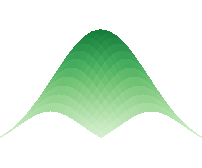
\includegraphics[height=\baselineskip]{pgfplotsedt}} PGFPlotsEdt \link{https://logcreative.github.io/PGFPlotsEdt/?lang=cn} 是一款基于 \pgfplots{} 的界面化绘图编辑器,基于 \faVuejs{} 开发。

  \note{当年是想做个跟 \TikZ{}Edt 类似的软件,用于快速生成统计图代码。也想过使用 Qt 写,当然后面放弃了,转向编写网页应用。当时本人还没有什么服务器,就写了个纯前端。}
\end{frame}

\begin{frame}
  \frametitle{PGFPlotsEdt 帮助我完成物理实验报告图...}
  \begin{columns}
    \begin{column}{0.25\textwidth}
      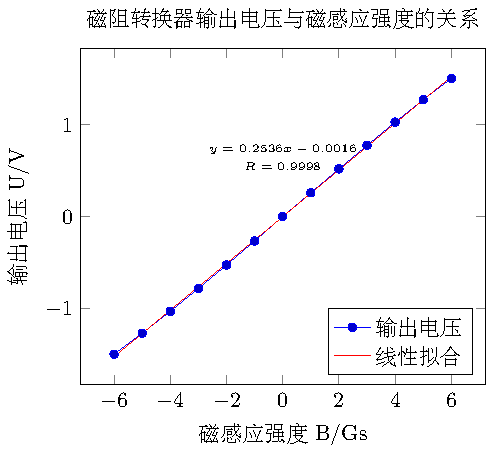
\includegraphics[width=\linewidth]{a}
      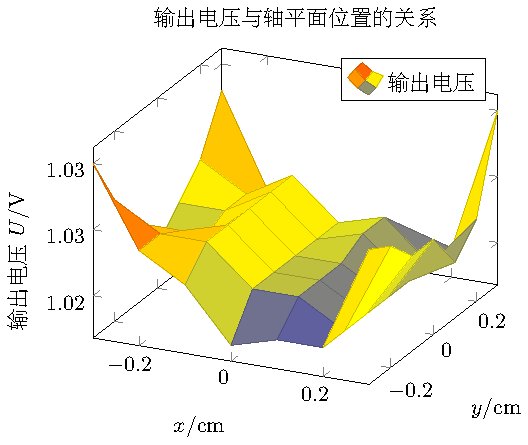
\includegraphics[width=\linewidth]{b}
    \end{column}
    \begin{column}{0.50\textwidth}
      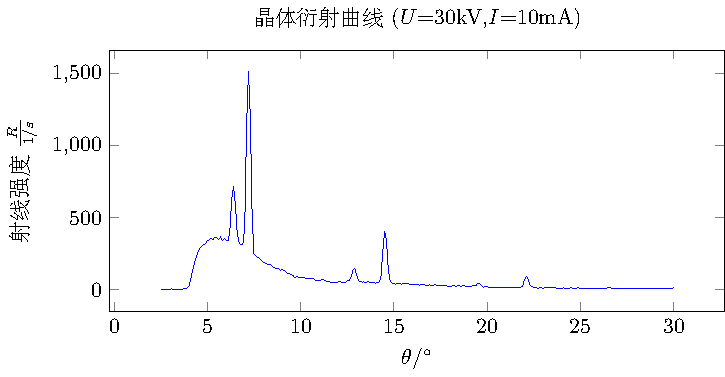
\includegraphics[width=\linewidth]{c}
      \begin{columns}
        \begin{column}{0.5\linewidth}
          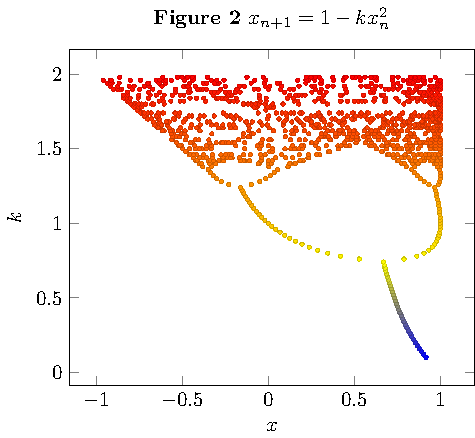
\includegraphics[width=\linewidth]{d}
        \end{column}
        \begin{column}{0.5\linewidth}
          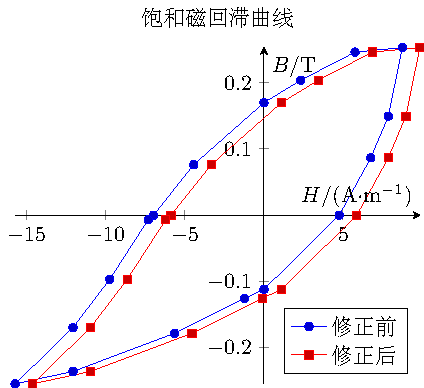
\includegraphics[width=\linewidth]{e}
        \end{column}
      \end{columns}
    \end{column}
    \begin{column}{0.25\textwidth}
      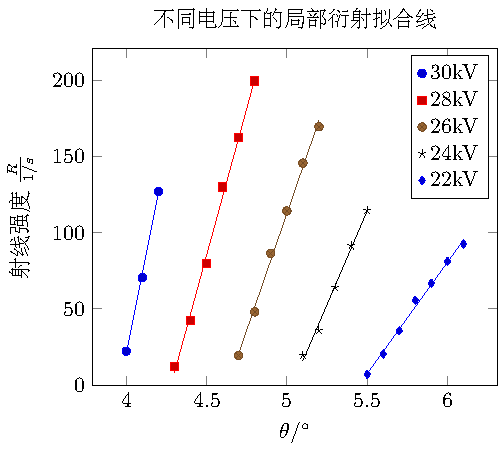
\includegraphics[width=\linewidth]{f}
      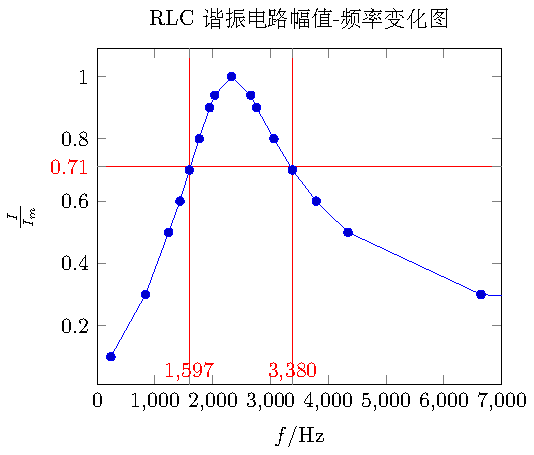
\includegraphics[width=\linewidth]{g}
    \end{column}
  \end{columns}
\end{frame}